\documentclass[12pt,a4paper]{article}
\usepackage[utf8]{inputenc}
\usepackage[T1]{fontenc}
\usepackage[polish]{babel}
\usepackage{lmodern}
\usepackage[a4paper,margin=2.0cm]{geometry}
\usepackage{amsmath,amssymb}
\usepackage{array,booktabs,longtable,multirow}
\usepackage{graphicx}
\usepackage{float}
\usepackage{enumitem}
\usepackage{fancyhdr}
\usepackage[hidelinks]{hyperref}
\usepackage{tikz}
\usetikzlibrary{positioning,arrows.meta}
\usepackage{xcolor}
\setlength{\parindent}{0pt}
\setlength{\parskip}{1.5pt}
\renewcommand{\arraystretch}{1.15}
\linespread{1.0}
\setlength{\abovedisplayskip}{6pt}
\setlength{\belowdisplayskip}{6pt}
\setlength{\abovedisplayshortskip}{4pt}
\setlength{\belowdisplayshortskip}{4pt}
\graphicspath{{./}}
\setlength{\headheight}{16pt}
\pagestyle{fancy}
\fancyhf{}
\lhead{Logika układów cyfrowych 2}
\rhead{Ćwiczenie 202(B)}
\cfoot{\thepage}
\newcommand{\linia}[1][6cm]{\rule{#1}{0.4pt}}
\newcommand{\xor}{\mathbin{\oplus}}
\newcommand{\xnor}{\mathbin{\odot}}
\newcommand{\img}[2][0.92\textwidth]{%
  \begin{figure}[H]\centering
  \includegraphics[width=#1,height=0.72\textheight,keepaspectratio]{#2}
  \end{figure}}
\begin{document}
\begin{titlepage}
\centering
\vspace*{0.28\textheight}
{\LARGE \textbf{Logika Układów Cyfrowych}\\[1.3cm]}
{\Large Dawid Kocyła i Ida Langowska\\[0.7cm]}
{\large 20 Październik 2025}
\end{titlepage}
\setcounter{tocdepth}{1}
\tableofcontents
\newpage
\section{Cel ćwiczenia}
Celem ćwiczenia było projektowanie i minimalizacja układów kombinacyjnych: komparatora, układu AND/OR, sumatorów, subtraktora, układów uzupełnienia do dwóch oraz detektora przedziału 5--10.
% ================================================================
\section{Zadanie 1 -- Komparator 2-bitowy}
\subsection{Treść zadania}
Zaprojektować komparator dwóch liczb 2-bitowych $A=A_1A_0$ oraz $B=B_1B_0$ w dwóch wariantach:
\begin{enumerate}[label=\alph*)]
\item dwa wyjścia: 00  $A=B$, 01  $A>B$, 10  $A<B$, 11 stan nieokreślony,
\item trzy wyjścia, z których każde odpowiada osobno relacji $A=B$, $A>B$ albo $A<B$.
\end{enumerate}
\subsection{Tabela prawdy}
\begin{center}
\small
\begin{tabular}{cccc|cc|ccc}
\toprule
$A_1$&$A_0$&$B_1$&$B_0$&$Y_1$&$Y_0$&$E$&$G$&$L$\\
\midrule
0&0&0&0&0&0&1&0&0\\
0&0&0&1&1&0&0&0&1\\
0&0&1&0&1&0&0&0&1\\
0&0&1&1&1&0&0&0&1\\
0&1&0&0&0&1&0&1&0\\
0&1&0&1&0&0&1&0&0\\
0&1&1&0&1&0&0&0&1\\
0&1&1&1&1&0&0&0&1\\
1&0&0&0&0&1&0&1&0\\
1&0&0&1&0&1&0&1&0\\
1&0&1&0&0&0&1&0&0\\
1&0&1&1&1&0&0&0&1\\
1&1&0&0&0&1&0&1&0\\
1&1&0&1&0&1&0&1&0\\
1&1&1&0&0&1&0&1&0\\
1&1&1&1&0&0&1&0&0\\
\bottomrule
\end{tabular}
\end{center}
W wariancie a) zachodzi $Y_0=G$ oraz $Y_1=L$.
\subsection{Minimalizacja}
\[
\begin{aligned}
E&=(\overline{A_1}\overline{B_1}+A_1B_1)
   (\overline{A_0}\overline{B_0}+A_0B_0)\\
 &= (A_1\xnor B_1)(A_0\xnor B_0).
\end{aligned}
\]
\[
\begin{aligned}
G&=A_1\overline{B_1}+(A_1B_1+\overline{A_1}\overline{B_1})A_0\overline{B_0}\\
 &=A_1(\overline{B_1}+A_0\overline{B_0})
   +\overline{B_1}A_0\overline{B_0}\\
 &=A_1\overline{B_1}+A_0A_1\overline{B_0}
   +A_0\overline{B_1}\overline{B_0}.
\end{aligned}
\]
\[
\begin{aligned}
L&=\overline{A_1}B_1+(A_1B_1+\overline{A_1}\overline{B_1})\overline{A_0}B_0\\
 &=B_1(\overline{A_1}+\overline{A_0}B_0)
   +\overline{A_1}\overline{A_0}B_0\\
 &=\overline{A_1}B_1+\overline{A_0}B_0B_1
   +\overline{A_1}\overline{A_0}B_0.
\end{aligned}
\]
Zastosowano $x+\overline{x}y=x+y$. Dla wariantu a):
\[
Y_0=G,\qquad Y_1=L.
\]
\subsection{Realizacja -- wariant a)}
Na rysunku przedstawiono realizację z dwoma wyjściami kodującymi wynik porównania.
\img{zadanie_1a.jpg}
\subsection{Realizacja -- wariant b)}
W wariancie b) zastosowano trzy niezależne wyjścia: $G$, $L$ i $E$.
\img{zadanie_1b.jpg}
\subsection{Weryfikacja}
Dla $(A,B)=(00,00)$ aktywne jest $E$, dla $(11,10)$ -- $G$, a dla $(01,10)$ -- $L$. W wariancie a) kod 11 nie występuje.
\subsection{Wnioski}
Trzy wyjścia wskazują relacje bezpośrednio; dwa pozwalają je zakodować mniejszą liczbą linii.
% ================================================================
\section{Zadanie 2 -- Układ realizujący sumę lub iloczyn logiczny}
\subsection{Treść zadania}
Zaprojektować układ, który w zależności od sygnału sterującego realizuje sumę logiczną lub iloczyn logiczny.
\subsection{Założenia i tabela prawdy}
Przyjęto:
\[
S=0\Rightarrow Y=A\cdot B,\qquad S=1\Rightarrow Y=A+B.
\]
\begin{center}
\begin{tabular}{ccc|c}
\toprule
$S$&$A$&$B$&$Y$\\
\midrule
0&0&0&0\\
0&0&1&0\\
0&1&0&0\\
0&1&1&1\\
1&0&0&0\\
1&0&1&1\\
1&1&0&1\\
1&1&1&1\\
\bottomrule
\end{tabular}
\end{center}
\subsection{Minimalizacja}
\[
\begin{aligned}
Y&=\overline{S}AB+S(A+B)\\
 &=\overline{S}AB+SA+SB\\
 &=AB+SA+SB=AB+S(A+B).
\end{aligned}
\]
Zastosowano $\overline{S}AB+SA=AB+SA$. Postać NAND--NAND:
\[
Y=\overline{\overline{AB}\cdot\overline{AS}\cdot\overline{BS}}.
\]
\subsection{Realizacja}
Schemat wykorzystuje bramki NAND. Trzy pierwsze bramki tworzą zanegowane iloczyny $AS$, $AB$ i $BS$, a ostatnia bramka NAND realizuje ich sumę zgodnie z prawem de Morgana.
\img[0.80\textwidth]{zadanie_2.jpg}
\subsection{Wnioski}
Sygnał $S$ wybiera AND lub OR; obie funkcje zrealizowano bramkami NAND.
% ================================================================
\section{Zadanie 3 -- Pełny sumator 1-bitowy}
\subsection{Treść zadania}
Zaprojektować pełny sumator 1-bitowy.
\subsection{Tabela prawdy}
\begin{center}
\begin{tabular}{ccc|cc}
\toprule
$A$&$B$&$C_{\mathrm{in}}$&$S$&$C_{\mathrm{out}}$\\
\midrule
0&0&0&0&0\\
0&0&1&1&0\\
0&1&0&1&0\\
0&1&1&0&1\\
1&0&0&1&0\\
1&0&1&0&1\\
1&1&0&0&1\\
1&1&1&1&1\\
\bottomrule
\end{tabular}
\end{center}
\subsection{Minimalizacja}
\[
\begin{aligned}
S&=\overline{A}\overline{B}C_{\mathrm{in}}
  +\overline{A}B\overline{C_{\mathrm{in}}}
  +A\overline{B}\overline{C_{\mathrm{in}}}+ABC_{\mathrm{in}}\\
 &=C_{\mathrm{in}}(\overline{A}\overline{B}+AB)
  +\overline{C_{\mathrm{in}}}(\overline{A}B+A\overline{B})\\
 &=(A\xor B)\xor C_{\mathrm{in}}.
\end{aligned}
\]
\[
\begin{aligned}
C_{\mathrm{out}}&=AB\overline{C_{\mathrm{in}}}+ABC_{\mathrm{in}}
 +A\overline{B}C_{\mathrm{in}}+\overline{A}BC_{\mathrm{in}}\\
 &=AB+C_{\mathrm{in}}(A\overline{B}+\overline{A}B)\\
 &=AB+C_{\mathrm{in}}(A\xor B)
  =AB+AC_{\mathrm{in}}+BC_{\mathrm{in}}.
\end{aligned}
\]
\subsection{Realizacja}
Dolna gałąź z dwiema bramkami XOR tworzy bit sumy. Górna część układu realizuje trzy iloczyny odpowiedzialne za przeniesienie, zapisane w strukturze NAND--NAND.
\img[0.85\textwidth]{zadanie_3.jpg}
\subsection{Wnioski}
Pełny sumator uwzględnia trzy bity wejściowe. Przeniesienie pojawia się wtedy, gdy co najmniej dwa z trzech wejść mają wartość 1.
% ================================================================
\section{Zadanie 4 -- Pełny subtraktor 1-bitowy}
\subsection{Treść zadania}
Zaprojektować pełny subtraktor 1-bitowy.
\subsection{Tabela prawdy}
\begin{center}
\begin{tabular}{ccc|cc}
\toprule
$A$&$B$&$B_{\mathrm{in}}$&$D$&$B_{\mathrm{out}}$\\
\midrule
0&0&0&0&0\\
0&0&1&1&1\\
0&1&0&1&1\\
0&1&1&0&1\\
1&0&0&1&0\\
1&0&1&0&0\\
1&1&0&0&0\\
1&1&1&1&1\\
\bottomrule
\end{tabular}
\end{center}
\subsection{Minimalizacja}
\[
\begin{aligned}
D&=\overline{A}\overline{B}B_{\mathrm{in}}
 +\overline{A}B\overline{B_{\mathrm{in}}}
 +A\overline{B}\overline{B_{\mathrm{in}}}+ABB_{\mathrm{in}}\\
 &=B_{\mathrm{in}}(\overline{A}\overline{B}+AB)
  +\overline{B_{\mathrm{in}}}(\overline{A}B+A\overline{B})\\
 &=(A\xor B)\xor B_{\mathrm{in}}.
\end{aligned}
\]
\[
\begin{aligned}
B_{\mathrm{out}}&=\overline{A}\overline{B}B_{\mathrm{in}}
 +\overline{A}B\overline{B_{\mathrm{in}}}
 +\overline{A}BB_{\mathrm{in}}+ABB_{\mathrm{in}}\\
 &=\overline{A}B+\overline{A}\overline{B}B_{\mathrm{in}}+ABB_{\mathrm{in}}\\
 &=\overline{A}B+\overline{A}B_{\mathrm{in}}+BB_{\mathrm{in}}.
\end{aligned}
\]
\subsection{Realizacja}
Bit różnicy jest generowany przez dwie bramki XOR. W torze pożyczki wykorzystano negację $A$ i strukturę NAND--NAND odpowiadającą powyższej funkcji.
\img[0.85\textwidth]{zadanie_4.jpg}
\subsection{Wnioski}
Różnicę wyznaczają bramki XOR, a pożyczkę -- funkcja uwzględniająca zanegowaną odjemną $A$.
% ================================================================
\section{Zadanie 5 -- 4-bitowy kaskadowy sumator równoległy}
\subsection{Treść zadania}
Z gotowych modułów zrealizować 4-bitowy kaskadowy sumator równoległy.
\subsection{Zasada działania}
Cztery pełne sumatory 1-bitowe połączono kaskadowo. Przeniesienie z pozycji mniej znaczącej jest wejściem przeniesienia kolejnego stopnia:
\[
(A_0,B_0,C_0)\rightarrow(S_0,C_1),
\]
\[
(A_1,B_1,C_1)\rightarrow(S_1,C_2),
\]
\[
(A_2,B_2,C_2)\rightarrow(S_2,C_3),
\]
\[
(A_3,B_3,C_3)\rightarrow(S_3,C_4).
\]
\subsection{Uproszczenie zależności}
\[
\begin{aligned}
P_i&=A_i\xor B_i,\qquad G_i=A_iB_i,\\
S_i&=P_i\xor C_i,\qquad C_{i+1}=G_i+P_iC_i,
\quad i=0,1,2,3.
\end{aligned}
\]
\subsection{Realizacja}
Na schemacie widać cztery identyczne stopnie pełnego sumatora oraz propagację przeniesienia od $C_0$ do $C_4$.
\img[0.72\textwidth]{zadanie_5.jpg}
\subsection{Przykładowa weryfikacja}
\begin{center}
\begin{tabular}{c|c|c|c}
\toprule
$A$&$B$&$C_0$&$C_4S_3S_2S_1S_0$\\
\midrule
0000&0000&0&00000\\
0011&0101&0&01000\\
1111&0001&0&10000\\
1010&0101&0&01111\\
0111&1000&1&10000\\
\bottomrule
\end{tabular}
\end{center}
\subsection{Wnioski}
Układ dodaje dwie liczby 4-bitowe i $C_0$. Propagacja przeniesienia przez kolejne stopnie zwiększa opóźnienie wyniku.
% ================================================================
\section{Zadanie 6 -- Uzupełnienie do dwóch z wykorzystaniem 7483}
\subsection{Treść zadania}
Za pomocą układu 7483 zrealizować układ generujący uzupełnienie do dwóch liczby 4-bitowej.
\subsection{Zasada działania}
Dla liczby 4-bitowej $A=A_3A_2A_1A_0$ uzupełnienie do dwóch wyznacza się z zależności
\[
Y=(\overline{A}+1)\bmod 16=(15-A+1)\bmod 16=(-A)\bmod 16.
\]
Do sumatora podaje się zanegowane bity $A$, $B=0000$ oraz $C_0=1$. Przeniesienie końcowe pomija się, zachowując wynik modulo 16.
\subsection{Realizacja}
Schemat przedstawia negację bitów wejściowych i dodanie jedynki za pomocą czterech kaskadowo połączonych sumatorów 1-bitowych.
\begin{figure}[H]
\centering
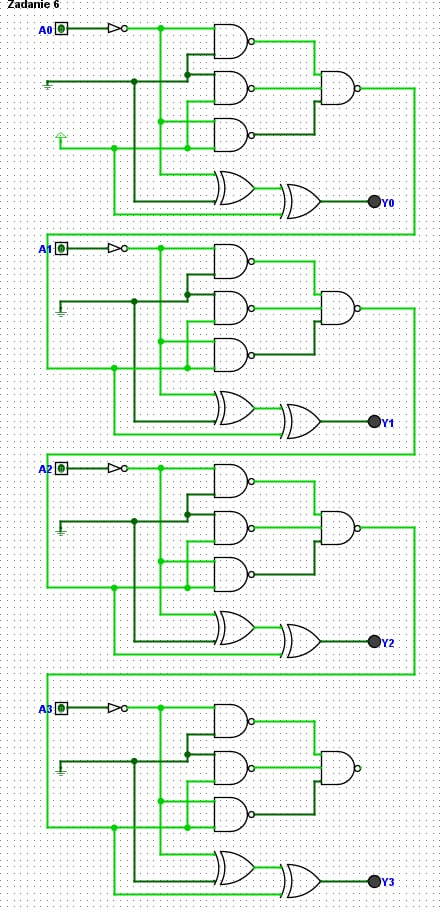
\includegraphics[width=0.72\textwidth,height=0.65\textheight,keepaspectratio]{zadanie_6.jpg}
\end{figure}
\subsection{Tabela testów}
\begin{center}
\begin{tabular}{c|c}
\toprule
$A$&$Y=\overline A+1$\\
\midrule
0000&0000\\
0001&1111\\
0010&1110\\
0101&1011\\
1000&1000\\
1111&0001\\
\bottomrule
\end{tabular}
\end{center}
\subsection{Wnioski}
Zanegowanie bitów i dodanie jedynki daje 4-bitowe uzupełnienie do dwóch.
% ================================================================
\section{Zadanie 7 -- Sterowane przepuszczenie lub negacja bitu}
\subsection{Treść zadania}
Zrealizować układ, który w zależności od sygnału sterującego daje na wyjściu sygnał wejściowy albo jego negację. Korzystając z takiego układu zaprojektować układ realizujący uzupełnienie do dwóch liczby 4-bitowej.
\subsection{Część A -- układ 1-bitowy}
Przyjęto, że $M=0$ oznacza przepuszczenie sygnału, a $M=1$ jego negację.
\begin{center}
\begin{tabular}{cc|c}
\toprule
$M$&$X$&$Y$\\
\midrule
0&0&0\\
0&1&1\\
1&0&1\\
1&1&0\\
\bottomrule
\end{tabular}
\end{center}
\textbf{Minimalizacja:}
\[
Y=\overline{M}X+M\overline{X}=X\xor M.
\]
Zatem pojedyncza bramka XOR realizuje dokładnie wymaganą funkcję.
\img[0.45\textwidth]{zadanie_7.jpg}
\subsection{Część B -- rozszerzenie do liczby 4-bitowej}
Cztery identyczne układy XOR można zastosować równolegle do wszystkich bitów. Aby otrzymać sterowaną negację arytmetyczną, do wyniku należy dodać sygnał $M$:
\[
Y=(A\xor M)+M,
\]
gdzie zapis $A\xor M$ oznacza wykonanie XOR każdego bitu $A_i$ z tym samym sygnałem $M$. Dla $M=0$ otrzymujemy $Y=A$, natomiast dla $M=1$:
\[
Y=\overline A+1,
\]
czyli uzupełnienie do dwóch (modulo 16).
Poniższy schemat przedstawia realizację układu 4-bitowego dla wejść $A_0$--$A_3$ i wyjść $Y_0$--$Y_3$.
\img[0.78\textwidth]{zadanie_7b.jpg}
\subsection{Przykładowa weryfikacja}
\begin{center}
\begin{tabular}{c|c|c}
\toprule
$M$&$A$&$Y$\\
\midrule
0&0101&0101\\
1&0101&1011\\
1&0000&0000\\
1&1111&0001\\
0&1010&1010\\
\bottomrule
\end{tabular}
\end{center}
\subsection{Wnioski}
Sterowanie XOR i przeniesieniem wejściowym pozwala uzyskać $Y=A$ dla $M=0$ lub uzupełnienie do dwóch dla $M=1$.
% ================================================================
\section{Zadanie 8 -- Detekcja liczby z przedziału 5--10}
\subsection{Treść zadania}
Zaprojektować układ, który sprawdza, czy 4-bitowa liczba wejściowa należy do przedziału 5--10. Można wykorzystać komparator scalony 7485.
\subsection{Tabela prawdy}
Przyjęto standardowo $X_3$ jako bit najbardziej znaczący, a $X_0$ jako najmniej znaczący.
\begin{center}
\begin{tabular}{c|cccc|c}
\toprule
wartość&$X_3$&$X_2$&$X_1$&$X_0$&$Y$\\
\midrule
0&0&0&0&0&0\\
1&0&0&0&1&0\\
2&0&0&1&0&0\\
3&0&0&1&1&0\\
4&0&1&0&0&0\\
5&0&1&0&1&1\\
6&0&1&1&0&1\\
7&0&1&1&1&1\\
8&1&0&0&0&1\\
9&1&0&0&1&1\\
10&1&0&1&0&1\\
11&1&0&1&1&0\\
12&1&1&0&0&0\\
13&1&1&0&1&0\\
14&1&1&1&0&0\\
15&1&1&1&1&0\\
\bottomrule
\end{tabular}
\end{center}
\subsection{Minimalizacja}
Dla kolejności zmiennych $X_3,X_2,X_1,X_0$:
\[
Y=\Sigma m(5,6,7,8,9,10).
\]
\[
\begin{aligned}
Y&=\overline{X_3}X_2
 (\overline{X_1}X_0+X_1\overline{X_0}+X_1X_0)\\
 &\quad+X_3\overline{X_2}
 (\overline{X_1}\overline{X_0}+\overline{X_1}X_0+X_1\overline{X_0})\\
 &=\overline{X_3}X_2(X_0+X_1\overline{X_0})
  +X_3\overline{X_2}(\overline{X_1}+X_1\overline{X_0})\\
 &=\overline{X_3}X_2(X_1+X_0)
  +X_3\overline{X_2}(\overline{X_1}+\overline{X_0})\\
 &=\overline{X_3}X_2X_0+\overline{X_3}X_2X_1\\
 &\quad+X_3\overline{X_2}\overline{X_0}
  +X_3\overline{X_2}\overline{X_1}.
\end{aligned}
\]
\subsection{Wersja A -- realizacja z bramek}
Cztery trójwejściowe bramki NAND tworzą zanegowane składniki iloczynowe, a końcowa bramka NAND wykonuje ich sumę zgodnie z prawem de Morgana.
\img{zadanie_8.jpg}
\subsection{Wersja B -- realizacja z komparatorami 7485}
Dwa komparatory 7485 sprawdzają granice przedziału:
\[
Y=(X\geq5)\cdot(X\leq10).
\]
Równoważnie można wykrywać stany spoza zakresu i zanegować ich sumę:
\[
Y=\overline{(X<5)+(X>10)}.
\]
Wejścia kaskadowe obu komparatorów ustawia się jako:
\[
I_{A>B}=0,\qquad I_{A<B}=0,\qquad I_{A=B}=1.
\]
Bramka NOR łączy wyjścia $X<5$ i $X>10$, dając $Y=1$ wyłącznie wewnątrz przedziału.
\img[0.95\textwidth]{zadanie_8b.jpg}
\subsection{Weryfikacja}
\begin{center}
\begin{tabular}{c|c}
\toprule
$X$&$Y$\\
\midrule
0100 (4)&0\\
0101 (5)&1\\
0111 (7)&1\\
1000 (8)&1\\
1010 (10)&1\\
1011 (11)&0\\
1111 (15)&0\\
\bottomrule
\end{tabular}
\end{center}
\subsection{Wnioski}
Wersja A (NAND--NAND) i wersja B (dwa komparatory 7485) wykrywają wartości od 5 do 10 włącznie.
% ================================================================
\section{Wnioski końcowe}
Tabele prawdy i zależności logiczne posłużyły do wyznaczenia funkcji realizowanych bramkami. Kaskadowe łączenie sumatorów umożliwiło dodawanie liczb 4-bitowych, a negacja bitów i dodanie jedynki -- wyznaczanie uzupełnienia do dwóch. Zastosowanie układu 7485 upraszcza realizację operacji arytmetycznych oraz porównywania liczb.
\end{document}
